\documentclass[11pt]{article}
\usepackage{fullpage}
\usepackage{amsthm}

\usepackage{amsthm,amsmath,amsfonts,amssymb,amstext,enumitem}
\usepackage{latexsym,ifthen,url,rotating,graphicx}
\usepackage{listings}
\usepackage{tikz}
\usetikzlibrary{arrows}
\usepackage{graphicx}
\usepackage[font=small,labelfont=bf]{caption}



% --- -----------------------------------------------------------------
% --- Document-specific definitions.
% --- -----------------------------------------------------------------
\lstset{
    columns=fixed,
    literate={—}{{---}}1 {…}{{...}}1
}

\newcommand{\todo}[1]{{\color{red}[TODO:{#1}]}}

\newtheorem{problem}{Problem}
\newtheorem{corollary}{Corollary}
\newtheorem{fact}{Fact}
\newtheorem{exercise}{Exercise}
\newtheorem{theorem}{Theorem}
\newtheorem{definition}{Definition}
\newtheorem{notation}{Notation}
\newtheorem{lemma}{Lemma}
\newtheorem{example}{Example}

\newcommand{\getsr}
  {{\:\stackrel{\raisebox{-2pt}{${\scriptscriptstyle \hspace{0.2em}\$}$}}
   {\leftarrow}\:}}
\newcommand{\points}[1]{\textbf{({#1} pts)}}

\newcommand{\Colon}{\ : \ }
\newcommand{\st}{\mathsf{state}}
\newcommand{\msgs}{\mathcal{M}}
\newcommand{\ctxts}{\mathcal{C}}
\newcommand{\keys}{\mathcal{K}}
\newcommand{\kg}{\mathcal{K}}
\newcommand{\enc}{E}
\newcommand{\dec}{E^{-1}}
\newcommand{\MAC}{\mathrm{MAC}}
\newcommand{\RMAC}{\mathrm{RMAC}}

\newcommand{\pk}{pk}
\newcommand{\sk}{sk}

\newcommand{\AES}{\mathsf{AES}}

\newcommand{\algorithm}[1]{\textbf{Alg} {#1}}

\newcommand{\calO}{\mathcal{O}}

\newcommand{\dlog}{\mathrm{dlog}}

\newcommand{\Adv}{\mathbf{Adv}}
\newcommand{\AdvPRF}[2]{\Adv^{\mathrm{prf}}_{#1}({#2})}
\newcommand{\AdvCPA}[2]{\Adv^{\mathrm{ind{-}cpa}}_{#1}({#2})}
\newcommand{\AdvCCA}[2]{\Adv^{\mathrm{ind{-}cca}}_{#1}({#2})}
\newcommand{\AdvKR}[2]{\Adv^{\mathrm{kr}}_{#1}({#2})}
\newcommand{\AdvCKR}[2]{\Adv^{\mathrm{ckr}}_{#1}({#2})}
\newcommand{\AdvRMR}[2]{\Adv^{\mathrm{rmr}}_{#1}({#2})}
\newcommand{\AdvCR}[2]{\Adv^{\mathrm{cr}}_{#1}({#2})}
\newcommand{\AdvUFCMA}[2]{\Adv^{\textrm{uf{-}cma}}_{#1}({#2})}
\newcommand{\AdvDL}[2]{\Adv^{\mathrm{dl}}_{#1}({#2})}

\newcommand{\Exp}{\mathbf{Exp}}
\newcommand{\ExpOW}[1]{\Exp^{\mathrm{ow}}({#1})}
\newcommand{\ExpCKR}[2]{\Exp^{\mathrm{ckr}}_{#1}({#2})}
\newcommand{\ExpRMR}[2]{\Exp^{\mathrm{rmr}}_{#1}({#2})}

\newcommand{\concat}{{\,\|\,}}
\newcommand{\xor}{\oplus}
\newcommand{\bits}{\{0,1\}}

\newcommand{\tcolh}{T^{\mathrm{col}}_h}
\newcommand{\tcolH}{T^{\mathrm{col}}_{H^2}}
\newcommand{\Hcomb}{H^{1\|2}}
\newcommand{\Hxor}{H^{1\oplus2}}

\newcommand{\EXP}{\textrm{EXP}}
\newcommand{\MODEXP}{\textrm{MOD{-}EXP}}
\newcommand{\ADD}{\textrm{ADD}}
\newcommand{\MULTIMODEXP}{\textrm{MULTI{-}MOD{-}EXP}}
\newcommand{\MUL}{\textrm{MUL}}
\newcommand{\MOD}{\textrm{MOD}}

\newcommand{\GG}{\mathbb{G}}
\newcommand{\ZZ}{\mathbb{Z}}

\newcommand{\rvrange}{\mathcal{R}}
\newcommand{\rspace}{\mathcal{C}}

\newcommand{\hatalpha}{\hat{\alpha}}


% --- -----------------------------------------------------------------
% --- Lecture notes formatting macros
% --- -----------------------------------------------------------------

%
% The following commands set up the lecnum (lecture number)
% counter and make various numbering schemes work relative
% to the lecture number.
%
\newcounter{lecnum}
%\renewcommand{\thepage}{\thelecnum-\arabic{page}}
\renewcommand{\thesection}{\thelecnum.\arabic{section}}
\renewcommand{\theexercise}{\thelecnum.\arabic{exercise}}
\renewcommand{\theexample}{\thelecnum.\arabic{example}}
\renewcommand{\thedefinition}{\thelecnum.\arabic{definition}}
\renewcommand{\theequation}{\thelecnum.\arabic{equation}}
\renewcommand{\thefigure}{\thelecnum.\arabic{figure}}
\renewcommand{\thefact}{\thelecnum.\arabic{fact}}
\renewcommand{\thetable}{\thelecnum.\arabic{table}}


%
% The following macro is used to generate the header.
%
\newcommand{\lecture}[2]{
   %\pagestyle{myheadings}
   %\thispagestyle{plain}
   \newpage
   \setcounter{lecnum}{#1}
   \setcounter{page}{1}
   \noindent
   \begin{center}
   \framebox{
      \vbox{\vspace{2mm}
    \hbox to 6.28in { {\bf CMSC 28400 Introduction to Cryptography
                        \hfill Autumn 2019} }
       \vspace{4mm}
       \hbox to 6.28in { {\Large \hfill #2 \hfill} }
       \vspace{2mm}
       \hbox to 6.28in { {\it Instructor: David Cash} \hfill }
      \vspace{2mm}}
   }
   \end{center}
   %\markboth{Lecture #1: #2}{Lecture #1: #2}
   \vspace*{4mm}
}





% --- -----------------------------------------------------------------
% --- The document starts here.
% --- -----------------------------------------------------------------
\begin{document}
%\lecture{**LECTURE-NUMBER**}{**DATE**}{**LECTURER**}{**SCRIBE**}
\lecture{2}{Notes \#2: Permutations and Enigma}

\tableofcontents

\noindent\hrulefill
\bigskip


These notes cover the permutation-based attack of Rejewski against the early
Enigma machines, along with some mathematical background used in the attack.

\section{The Simplified Enigma Machine} 

We will study a somewhat simplified version of the Enigma machine used in early
1930s. In Figure~\ref{fig:photos} two versions of the Enigma are pictured.  The
relevant parts of the machine are a keyboard, a light-board, a plug-board, and
a rotor assembly consisting of three rotors along with a special
\emph{reflector} (not visible). The rotors are electrical implementations of a
substitution cipher on $\Sigma=\{\mathtt{A},\ldots,\mathtt{Z}\}$: They have 26
connections (with labels) on each side, and in between is a mess of wires that
physically permutes how they are connected.  The rotors are designed to be
chained together, and also so that they can rotate to change how their 26
connections line up. The rotors are also designed so their their rotational
position is externally visible after they are placed in the machine, and they
can be manually rotated in discrete $1/26$\textsuperscript{th} steps.

An Enigma user would actually have several rotors stored in a box, but only
three would be used at a time (in this version; other rotor-based ciphers and
later Enigmas had more than three rotors).

To operate these machines, one would start by configuring the machine according
to the \emph{day key} which were distributed to everyone in order for them to
communicate. These settings included which rotors to use, how to align them
with respect to the rest of the machine, which connections to make on the
plugboard, as well as something called the \emph{ring setting} that we will
ignore.

\begin{figure}[ht]
    \begin{center}
        \begin{tabular}{cc}
            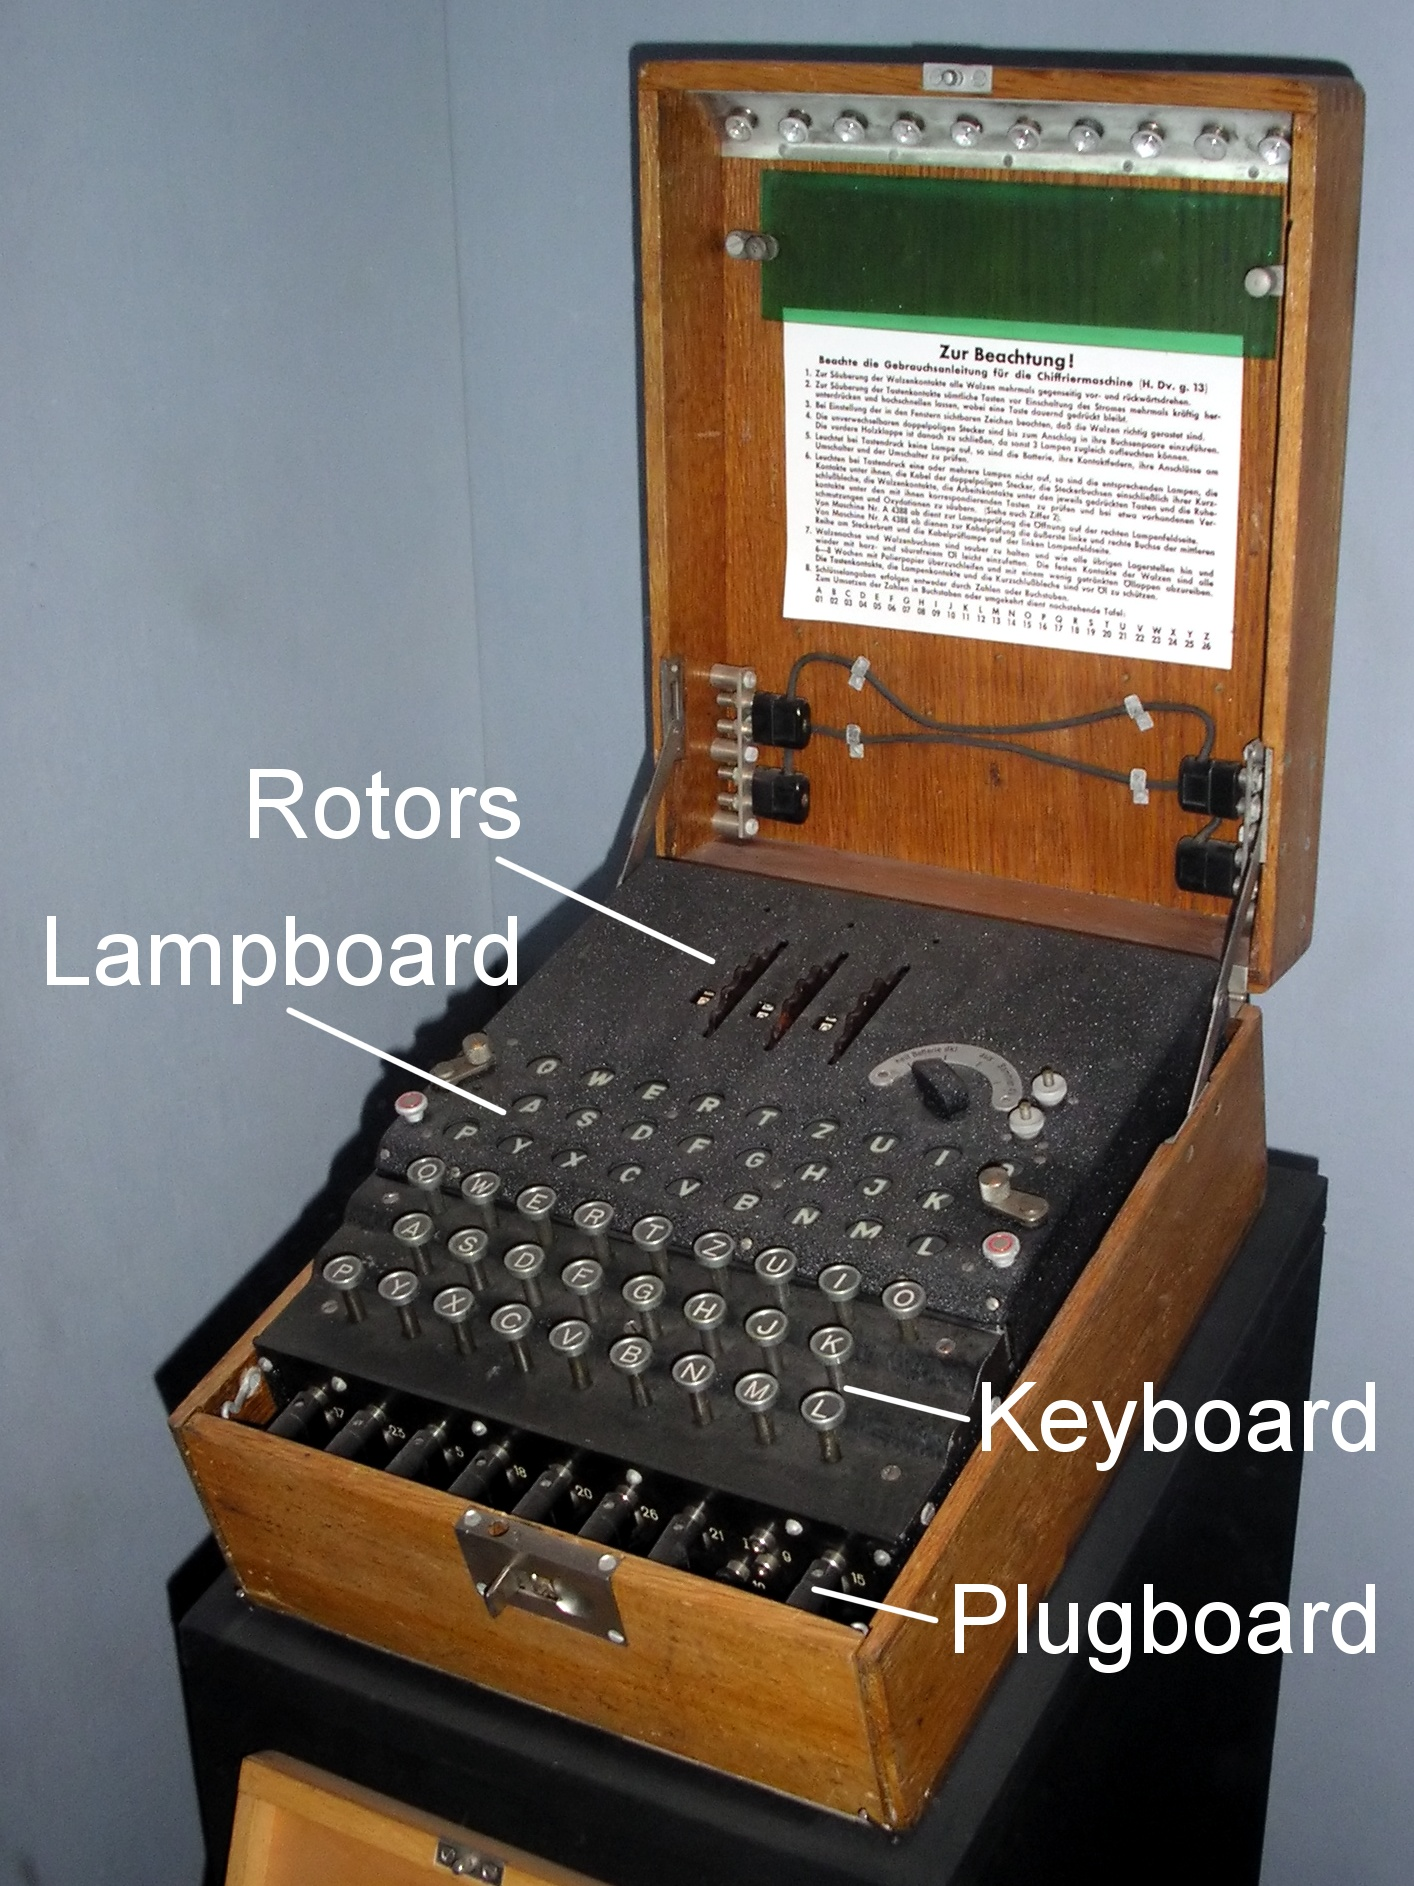
\includegraphics[width=6cm]{enigma-case.jpg}
            &
            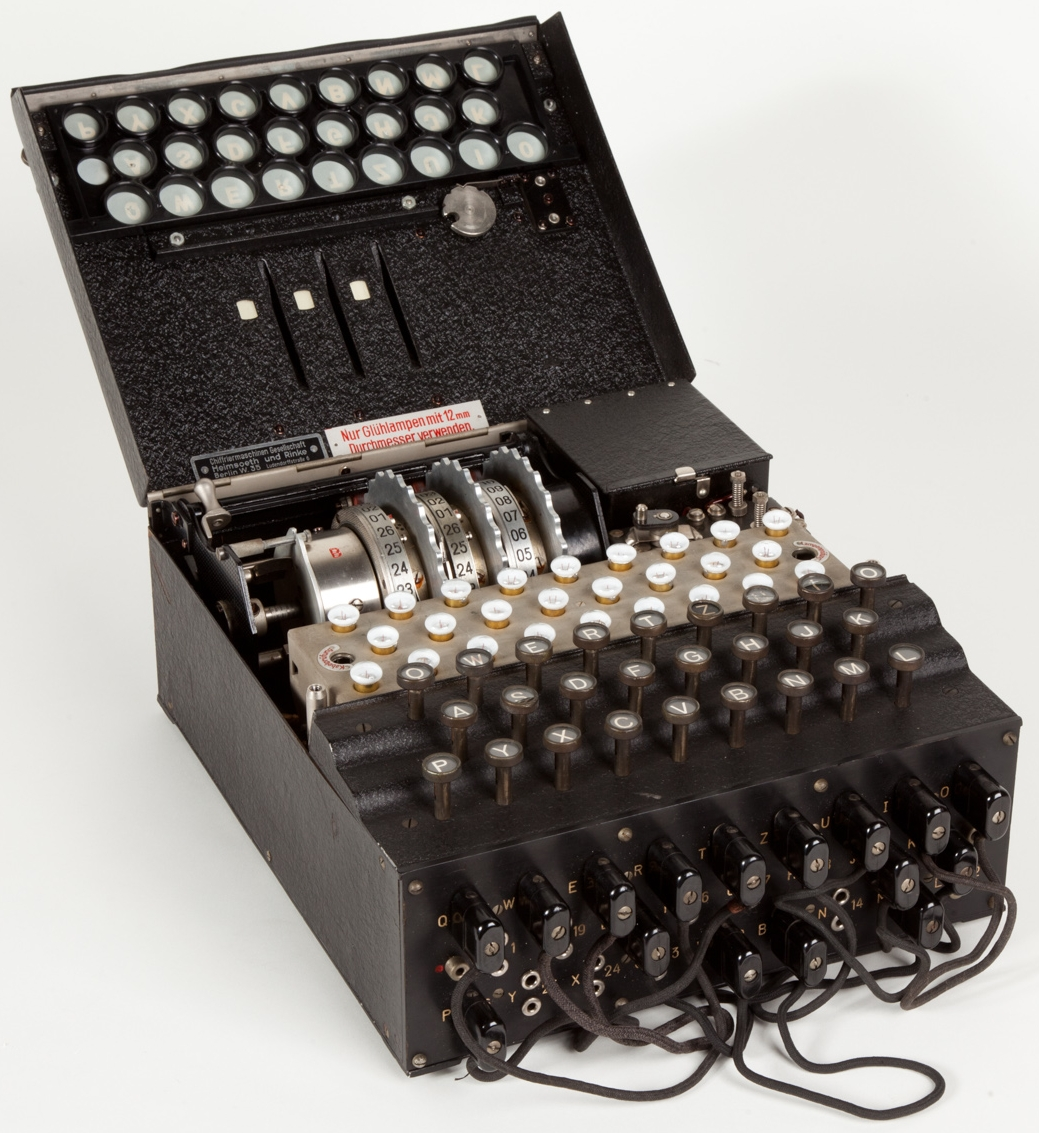
\includegraphics[width=6cm]{enigma-no-case.jpg}
        \end{tabular}
    \end{center}
    \caption{Two images of Enigma. Credit: Left image by Karsten Sperling (public domain, downloaded at \protect\url{https://commons.wikimedia.org/wiki/File:EnigmaMachineLabeled.jpg}, Right image by Alessandro Nassiri (\protect\url{https://creativecommons.org/licenses/by-sa/4.0/deed.en}, no changes.)}
    \label{fig:photos}
\end{figure}

Once configured, the operation is simple: To encipher a letter one presses a
key on the keyboard. A electric signal passes from the keyboard through the
plugboard, three rotors, the reflector, and then through the rotors again and
the plugboard again before lighting up a letter on the lightboard, which is the
enciphered letter. This is partially diagrammed in top part of
Figure~\ref{fig:enigma}, which is drawn as if the Enigma does not have a
plugboard. We note that the reflector is always wired to avoid ever mapping
a letter to itself.

The force of pressing the key would also rotate the rotors. The right-most
``first'' rotor will always rotate, and the other two rotors will rotate on a
schedule depending on the positioning of a physical catch between the rotors.
In these notes, we'll work under the assumption that only the first rotor
moves. The effect of a rotating on the electrical connections is diagramed
in the bottom of Figure~\ref{fig:enigma}.



\begin{figure}[h]
\begin{center}
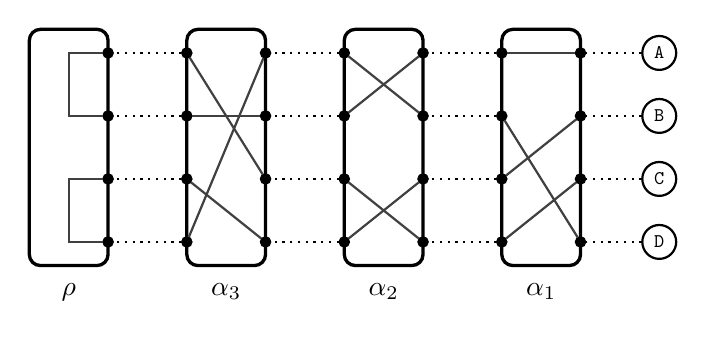
\begin{tikzpicture}
    \tikzstyle{connect}=[circle, draw, thin,fill=black, scale=0.4]
    \tikzstyle{every path}=[thick]
    \tikzstyle{rotor}=[very thick, rounded corners]
    \tikzstyle{input}=[circle,draw,scale=.7]
    \tikzstyle{internalwire}=[thick,darkgray]
    
    % rotors
    \draw[rotor] (0,0) rectangle (1,3);
    \node[below] at (.5,-.1) {$\rho$};
    \draw[rotor] (2,0) rectangle (3,3);
    \node[below] at (2.5,-.1) {$\alpha_3$};
    \draw[rotor] (4,0) rectangle (5,3);
    \node[below] at (4.5,-.1) {$\alpha_2$};
    \draw[rotor] (6,0) rectangle (7,3);
    \node[below] at (6.5,-.1) {$\alpha_1$};

    % first rotor nodes
    \node[connect] (r1r1) at (7,2.7) {};
    \node[connect] (r1r2) at (7,1.9) {};
    \node[connect] (r1r3) at (7,1.1) {};
    \node[connect] (r1r4) at (7,.3) {};
    \node[connect] (r1l1) at (6,2.7) {};
    \node[connect] (r1l2) at (6,1.9) {};
    \node[connect] (r1l3) at (6,1.1) {};
    \node[connect] (r1l4) at (6,.3) {};
    % first rotor wires
    \draw[internalwire] (r1r1) to (r1l1);
    \draw[internalwire] (r1r2) to (r1l3);
    \draw[internalwire] (r1r3) to (r1l4);
    \draw[internalwire] (r1r4) to (r1l2);

    % second rotor nodes
    \node[connect] (r2r1) at (5,2.7) {};
    \node[connect] (r2r2) at (5,1.9) {};
    \node[connect] (r2r3) at (5,1.1) {};
    \node[connect] (r2r4) at (5,.3) {};
    \node[connect] (r2l1) at (4,2.7) {};
    \node[connect] (r2l2) at (4,1.9) {};
    \node[connect] (r2l3) at (4,1.1) {};
    \node[connect] (r2l4) at (4,.3) {};
    % second rotor wires
    \draw[internalwire] (r2r1) to (r2l2);
    \draw[internalwire] (r2r2) to (r2l1);
    \draw[internalwire] (r2r3) to (r2l4);
    \draw[internalwire] (r2r4) to (r2l3);

    % third rotor nodes
    \node[connect] (r3r1) at (3,2.7) {};
    \node[connect] (r3r2) at (3,1.9) {};
    \node[connect] (r3r3) at (3,1.1) {};
    \node[connect] (r3r4) at (3,.3) {};
    \node[connect] (r3l1) at (2,2.7) {};
    \node[connect] (r3l2) at (2,1.9) {};
    \node[connect] (r3l3) at (2,1.1) {};
    \node[connect] (r3l4) at (2,.3) {};
    % third rotor wires
    \draw[internalwire] (r3r1) to (r3l4);
    \draw[internalwire] (r3r2) to (r3l2);
    \draw[internalwire] (r3r3) to (r3l1);
    \draw[internalwire] (r3r4) to (r3l3);  

    % reflector nodes
    \node[connect] (rfr1) at (1,2.7) {};
    \node[connect] (rfr2) at (1,1.9) {};
    \node[connect] (rfr3) at (1,1.1) {};
    \node[connect] (rfr4) at (1,.3) {};
    % reflector wires
    \draw[internalwire] (rfr1) -- (.5,2.7) -- (.5,1.9) -- (rfr2);
    \draw[internalwire] (rfr3) -- (.5,1.1) -- (.5,.3) -- (rfr4);

    % input letters
    \node[input] (Ain) at (8,2.7) {$\mathtt{A}$};
    \node[input] (Bin) at (8,1.9) {$\mathtt{B}$};
    \node[input] (Cin) at (8,1.1) {$\mathtt{C}$};
    \node[input] (Din) at (8,.3) {$\mathtt{D}$};

    % connecting wires
    \draw[dotted] (r1l1) -- (r2r1);
    \draw[dotted] (r1l2) -- (r2r2);
    \draw[dotted] (r1l3) -- (r2r3);
    \draw[dotted] (r1l4) -- (r2r4);

    \draw[dotted] (r2l1) -- (r3r1);
    \draw[dotted] (r2l2) -- (r3r2);
    \draw[dotted] (r2l3) -- (r3r3);
    \draw[dotted] (r2l4) -- (r3r4);

    \draw[dotted] (r3l1) -- (rfr1);
    \draw[dotted] (r3l2) -- (rfr2);
    \draw[dotted] (r3l3) -- (rfr3);
    \draw[dotted] (r3l4) -- (rfr4);

    \draw[dotted] (Ain) -- (r1r1);
    \draw[dotted] (Bin) -- (r1r2);
    \draw[dotted] (Cin) -- (r1r3);
    \draw[dotted] (Din) -- (r1r4);

\end{tikzpicture}

\vspace{.15in}

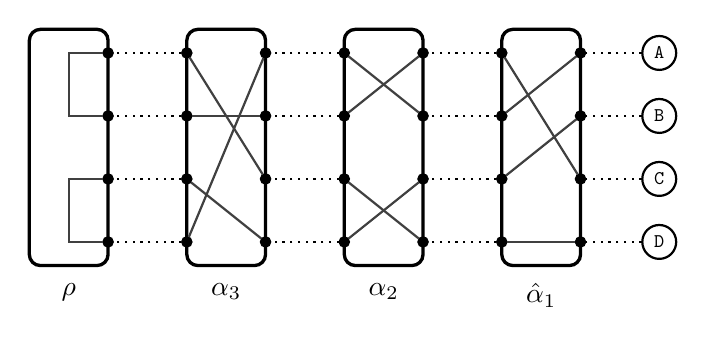
\begin{tikzpicture}
    \tikzstyle{connect}=[circle, draw, thin,fill=black, scale=0.4]
    \tikzstyle{every path}=[thick]
    \tikzstyle{rotor}=[very thick, rounded corners]
    \tikzstyle{input}=[circle,draw,scale=.7]
    \tikzstyle{internalwire}=[thick,darkgray]
    
    % rotors
    \draw[rotor] (0,0) rectangle (1,3);
    \node[below] at (.5,-.1) {$\rho$};
    \draw[rotor] (2,0) rectangle (3,3);
    \node[below] at (2.5,-.1) {$\alpha_3$};
    \draw[rotor] (4,0) rectangle (5,3);
    \node[below] at (4.5,-.1) {$\alpha_2$};
    \draw[rotor] (6,0) rectangle (7,3);
    \node[below] at (6.5,-.1) {$\hatalpha_1$};

    % first rotor nodes
    \node[connect] (r1r1) at (7,2.7) {};
    \node[connect] (r1r2) at (7,1.9) {};
    \node[connect] (r1r3) at (7,1.1) {};
    \node[connect] (r1r4) at (7,.3) {};
    \node[connect] (r1l1) at (6,2.7) {};
    \node[connect] (r1l2) at (6,1.9) {};
    \node[connect] (r1l3) at (6,1.1) {};
    \node[connect] (r1l4) at (6,.3) {};
    % first rotor wires
    \draw[internalwire] (r1r1) to (r1l2);
    \draw[internalwire] (r1r2) to (r1l3);
    \draw[internalwire] (r1r3) to (r1l1);
    \draw[internalwire] (r1r4) to (r1l4);

    % second rotor nodes
    \node[connect] (r2r1) at (5,2.7) {};
    \node[connect] (r2r2) at (5,1.9) {};
    \node[connect] (r2r3) at (5,1.1) {};
    \node[connect] (r2r4) at (5,.3) {};
    \node[connect] (r2l1) at (4,2.7) {};
    \node[connect] (r2l2) at (4,1.9) {};
    \node[connect] (r2l3) at (4,1.1) {};
    \node[connect] (r2l4) at (4,.3) {};
    % second rotor wires
    \draw[internalwire] (r2r1) to (r2l2);
    \draw[internalwire] (r2r2) to (r2l1);
    \draw[internalwire] (r2r3) to (r2l4);
    \draw[internalwire] (r2r4) to (r2l3);

    % third rotor nodes
    \node[connect] (r3r1) at (3,2.7) {};
    \node[connect] (r3r2) at (3,1.9) {};
    \node[connect] (r3r3) at (3,1.1) {};
    \node[connect] (r3r4) at (3,.3) {};
    \node[connect] (r3l1) at (2,2.7) {};
    \node[connect] (r3l2) at (2,1.9) {};
    \node[connect] (r3l3) at (2,1.1) {};
    \node[connect] (r3l4) at (2,.3) {};
    % third rotor wires
    \draw[internalwire] (r3r1) to (r3l4);
    \draw[internalwire] (r3r2) to (r3l2);
    \draw[internalwire] (r3r3) to (r3l1);
    \draw[internalwire] (r3r4) to (r3l3);  

    % reflector nodes
    \node[connect] (rfr1) at (1,2.7) {};
    \node[connect] (rfr2) at (1,1.9) {};
    \node[connect] (rfr3) at (1,1.1) {};
    \node[connect] (rfr4) at (1,.3) {};
    % reflector wires
    \draw[internalwire] (rfr1) -- (.5,2.7) -- (.5,1.9) -- (rfr2);
    \draw[internalwire] (rfr3) -- (.5,1.1) -- (.5,.3) -- (rfr4);

    % input letters
    \node[input] (Ain) at (8,2.7) {$\mathtt{A}$};
    \node[input] (Bin) at (8,1.9) {$\mathtt{B}$};
    \node[input] (Cin) at (8,1.1) {$\mathtt{C}$};
    \node[input] (Din) at (8,.3) {$\mathtt{D}$};

    % connecting wires
    \draw[dotted] (r1l1) -- (r2r1);
    \draw[dotted] (r1l2) -- (r2r2);
    \draw[dotted] (r1l3) -- (r2r3);
    \draw[dotted] (r1l4) -- (r2r4);

    \draw[dotted] (r2l1) -- (r3r1);
    \draw[dotted] (r2l2) -- (r3r2);
    \draw[dotted] (r2l3) -- (r3r3);
    \draw[dotted] (r2l4) -- (r3r4);

    \draw[dotted] (r3l1) -- (rfr1);
    \draw[dotted] (r3l2) -- (rfr2);
    \draw[dotted] (r3l3) -- (rfr3);
    \draw[dotted] (r3l4) -- (rfr4);

    \draw[dotted] (Ain) -- (r1r1);
    \draw[dotted] (Bin) -- (r1r2);
    \draw[dotted] (Cin) -- (r1r3);
    \draw[dotted] (Din) -- (r1r4);

\end{tikzpicture}
\end{center}
\caption{A diagram of the electrical connections in an Enigma without a
plugboard, for the alphabet
$\Sigma=\{\mathtt{A},\mathtt{B},\mathtt{C},\mathtt{D}\}$.
The top diagram shows an initial configuration, while the bottom
shows the configuration after the right rotor rotates by one step (upwards
in the diagram). The labeling will be discussed later.}
\label{fig:enigma}
\end{figure}

\subsection{Message Keys and Rejewski's Attack}

It was recognized that if everyone were to set their Enigma to same day key and
then encipher messages, than basic frequency analysis would defeat the
encryption (since the same permutation would be applied to
$i$\textsuperscript{th} letter by everyone).  

In the early usage of the Enigma, this was mitigated by using \emph{message
keys}. The sender would choose a random three-letter message key $xyz$.
The sender would then begin the transmission by enciphering the letters
$xyz$ \emph{twice}. After this, the sender would manually rotate the
rotors to positions $x,y,z$, and then encipher the payload of the message
as before.

\begin{example}
    Suppose the sender chooses message key $\mathtt{TAQ}$. The sender enciphers
    the messages twice using the day key; Suppose this produces the six letters
    $\mathtt{ICPWLV}$. The sender then resets the three rotors to positions
    $\mathtt{T}$,$\mathtt{A}$, and $\mathtt{Q}$, and then enciphers the
    rest of the message.
\end{example}

The idea was that message keys would provide enough randomization to defeat
frequency analysis. However, it did not work against more clever attacks.
Specifically, we will show that given many ciphertexts (about fifty in
practice), a clever attack easily recovers all of the message keys!  Thus if
one know the day keys (say by stealing them), then all messages can be
decrypted. 

\section{Permutations and Cycle Decompositions}

Our first order of business will be to give a clear and useful mathematical
description of an Enigma machine. The most useful language for doing so turns
out to be \emph{permutations}, which we turn to in the next section before
returning to the attack later.


\begin{definition}
    A \emph{permutation on a set $\Sigma$} is a one-to-one and onto
    function from $\Sigma$ to itself.
\end{definition}
Recall that \emph{one-to-one} means that $x\neq y$ implies $\pi(x)\neq \pi(y)$,
and \emph{onto} means that for every $y\in\Sigma$ there exists $x\in\Sigma$
such that $\pi(x)=y$.

Here are two examples of permutations on the set $\Sigma=\{1,2,3,4,5,6\}$.
They are presented in ``table form'', so given $x$ we can simply look
up $\pi(x)$.
\begin{center}
        \begin{tabular}{cc}
            \begin{minipage}{2in}
                \begin{tabular}{c|*{7}c}
                    $x$      & 1 & 2 & 3 & 4 & 5 & 6 \\ \hline
                    $\pi(x)$ & 4 & 1 & 6 & 5 & 2 & 3
                \end{tabular}
            \end{minipage}
            and
            &
            \begin{minipage}{2in}
                \begin{tabular}{c|*{7}c}
                    $x$         & 1 & 2 & 3 & 4 & 5 & 6 \\ \hline
                    $\sigma(x)$ & 2 & 1 & 5 & 4 & 6 & 3
                \end{tabular}.
            \end{minipage}
        \end{tabular}
        \end{center}

\begin{exercise}
    Suppose $\Sigma$ is finite. Show that any one-to-one function
    $\pi:\Sigma\to\Sigma$ is a permutation. Do the same for any
    onto function.

    Show that neither of these hold in general when $\Sigma$ is infinite
    by finding a counterexample. (We won't need permutations on
    infinite sets again in this class.)
\end{exercise}

We will write $\pi\sigma$ for the composition of $\pi$ and $\sigma$ (where
we mean: ``first apply to $\sigma$, then apply $\pi$''). So in table
notation $\pi\sigma$ is
\begin{center}
    \begin{minipage}{2in}
        \begin{tabular}{c|*{7}c}
            $x$            & 1 & 2 & 3 & 4 & 5 & 6 \\ \hline
            $\pi\sigma(x)$ & 1 & 4 & 2 & 5 & 3 & 6
        \end{tabular}.
    \end{minipage}
\end{center}
If $\pi\sigma = \sigma\pi$ then we say that \emph{$\pi$ and $\sigma$ commute}.


We write $\pi^{-1}$ for the inverse of $\pi$; You can prove that
$\pi^{-1}$ is also a permutation. The inverse $\pi^{-1}$ for our example
is given in table form as:
\begin{center}
    \begin{minipage}{2in}
        \begin{tabular}{c|*{7}c}
            $x$            & 1 & 2 & 3 & 4 & 5 & 6 \\ \hline
            $\pi^{-1}(x)$  & 2 & 5 & 6 & 1 & 4 & 3
        \end{tabular}.
    \end{minipage}
\end{center}
For any permutation $\pi$, the product $\pi\pi^{-1}$ is always the
\emph{identity permutation} $e:\Sigma\to\Sigma$ defined by $e(x)=x$.
\begin{exercise}
    Show by induction on $t$ 
    \[
        (\pi_1\cdots\pi_t)^{-1}
        =  \pi_t^{-1}\cdots\pi_1^{-1}
    \]
    for any permutations $\pi_1,\ldots,\pi_t$.
\end{exercise}

\subsection{Cycles in Permutations}

The table setting is intuitive, but the real structure of permutations
is revealed if we use them to create a graph, as follows. Let $\pi$
be a permutation on $\Sigma$, and define a directed
graph $G_\pi = (V,E)$ with vertex set $V=\Sigma$ and an edge from
each $x\in\Sigma$ to $\pi(x)$. For example, here is the graph
$G_\pi$ created from the table above:
\begin{center}
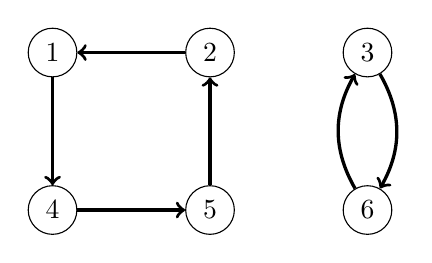
\begin{tikzpicture}
    \tikzset{vertex/.style = {shape=circle,draw}}
    \tikzset{edge/.style = {->,very thick}}
    % vertices
    \node[vertex] (1) at  (-2,1) {$1$};
    \node[vertex] (2) at  (0,1) {$2$};
    \node[vertex] (3) at  (2,1) {$3$};
    \node[vertex] (4) at  (-2,-1) {$4$};
    \node[vertex] (5) at (0,-1) {$5$};
    \node[vertex] (6) at (2,-1) {$6$};
    %edges
    \draw[edge] (1) to (4);
    \draw[edge] (2) to (1);
    \draw[edge] (3) to[bend left] (6);
    \draw[edge] (4) to (5);
    \draw[edge] (5) to (2);
    \draw[edge] (6) to[bend left] (3);
\end{tikzpicture}
\end{center}
And here is the graph for $G_\sigma$:
\begin{center}
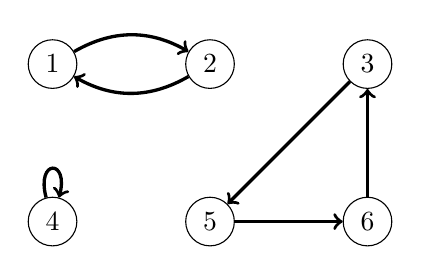
\begin{tikzpicture}
    \tikzset{vertex/.style = {shape=circle,draw}}
    \tikzset{edge/.style = {->,very thick}}
    % vertices
    \node[vertex] (1) at  (-2,1) {$1$};
    \node[vertex] (2) at  (0,1) {$2$};
    \node[vertex] (3) at  (2,1) {$3$};
    \node[vertex] (4) at  (-2,-1) {$4$};
    \node[vertex] (5) at (0,-1) {$5$};
    \node[vertex] (6) at (2,-1) {$6$};
    %edges
    \draw[edge] (1) to[bend left] (2);
    \draw[edge] (2) to[bend left] (1);
    \draw[edge] (3) to (5);
    \draw[edge] (4) to[loop above] (4);
    \draw[edge] (5) to (6);
    \draw[edge] (6) to (3);
\end{tikzpicture}
\end{center}
What these graphs have in common is that \emph{every node is a member of
exactly one directed cycle} (which may be a self loop). Indeed this will be
true for \emph{any} permutation on a finite set: Start from any node and
iteratively apply the permutation to walk on nodes. Since the set is
finite, you must eventually repeat a node. Since the permutation is
one-to-one, the first repetition must bring you back to where you started.
Starting at another node not on this cycle will generate yet another
cycle, and so on. The upshot is: 
\emph{There is a one-to-one
correspondence between permutations on $\Sigma$ and graphs that consist of a
covering of all of $\Sigma$ with directed cycles}.

This structure motivates the following notation:
\begin{definition}
    We write $(a_1\ a_2\ \cdots\ a_t)$, where all of the $a_i\in\Sigma$,
    for the permutation on $\Sigma$ that maps $a_1$ to $a_2$,
    $a_2$ to $a_3$, etc, $a_t$ to $a_1$, and for the rest
    of the $x\in\Sigma$ maps $x$ to itself.
\end{definition}
We use this notation combined with our product notation. So for example $\pi =
(1\ 4\ 5\ 2)(3\ 6)$ is another way of writing $\pi$ from above, which can be
checked by hand (and of course, the notation still means that we apply the
permutation $(3\ 6)$ first, and then permutation $(1\ 4\ 5\ 2)$. 

\begin{exercise}
    Call two cycles $(a_1\ a_2\ \ldots)$ and $(b_1\ b_2\ \ldots)$
    \emph{disjoint} if the sets $\{a_1,a_2,\ldots\}$ and $\{b_1,b_2,\ldots\}$
    are disjoint.  Show that disjoint cycles commute.
\end{exercise}

Permutations can be written as a product of cycles in several ways. For
example, we can check that $(1\ 4)(1\ 4\ 5\ 2)= (2\ 4\ 5)$. However,
if we require that cycles be \emph{disjoint}, then there is essentially
only one way to express the permutation.
\begin{theorem}
    Every permutation on a finite set $\Sigma$ can be written as a
    product of disjoint cycles. Moreover, this product is unique up
    to ordering the cycles and rotating elements within cycles.
\end{theorem}
We will not prove this theorem formally, but if one accepts the equivalence
between graphs of cycles and permutations then it is very intuitive; The cycles
in the product expression of $\pi$ correspond to the cycles of the graph, and
the order of the cycles or how they are rotated does not affect the
corresponding graph.


As an example  of the theorem in action,
$\pi = (1\ 4\ 5\ 2)(3\ 6)$ is a product of disjoint cycles, and
\[
    \pi 
    = (1\ 4\ 5\ 2)(3\ 6)
    = (3\ 6)(1\ 4\ 5\ 2)
    = (6\ 3)(1\ 4\ 5\ 2)
    = (6\ 3)(5\ 2\ 1\ 4) = \ldots
\]
and so on all are all equal $\pi$; These are the \emph{only} ways to write
$\pi$ as a product of disjoint cycles. We shall refer to these ways
(collectively) as \emph{the} cycle decomposition of $\pi$, with the
understanding that it is not exactly unique (only sort-of-unique).

It is important to remember that every element not appearing in a cycle is
assumed to be fixed by the permutation; So in effect there are often extra
unwritten cycles of length $1$ hanging around.

\begin{definition}
    Let $\pi$ be a permutation on $\Sigma$. We say that $\pi$ has \emph{type}
    $[1^{z_1} 2^{z_2}\cdots n^{z_n}]$ if for all $i=1,\ldots,n$, the
    cycle decomposition of $\pi$ has exactly $z_i$ cycles of length $i$.
\end{definition}
When some $z_i=0$ we omit $i^{z_i}$ from the notation.

It takes a moment to verify that this definition is ``well defined'', which
means that we if take \emph{any} way of writing $\pi$ as a disjoint product of
cycles, and check their lengths, we will get the same type. For example, our
$\pi$ has type $[2^14^1]$, and it does not matter which ordering or rotations
of the cycles we take.

\begin{example} Let $\Sigma = \{1,2,3,4,5,6\}$.
    \begin{itemize}
        \item The permutation $(1\ 2)(3\ 4)(5\ 6)$ has type $[2^3]$.
        \item The permutation $(1\ 2\ 3\ 4)$ has type $[1^24^1]$.
        \item The permutation $(1\ 4\ 3)(5\ 6)$ has type $[1^12^13^1]$.
    \end{itemize}
\end{example}

\subsection{Conjugates of Permutations}

The structure of the Enigma machine can be simplified by introducing
the concept of \emph{conjugates} of permutations.

\begin{definition}
    Let $\pi,\sigma$ be permutations on $\Sigma$. The \emph{conjugate of
    $\sigma$ by $\pi$} is defined to be the permutation
    $\pi\sigma\pi^{-1}$.
\end{definition}

\begin{theorem}
    Let $\sigma$ have cycle decomposition $(a_1\ a_2\ \ldots)(b_1\ b_2\
    \ldots)\cdots$. Then the conjugate $\pi\sigma\pi^{-1}$ has cycle
    decomposition
    \[
        (\pi(a_1)\ \pi(a_2)\ \ldots)(\pi(b_1)\ \pi(b_2)\ \ldots)\cdots.
    \]
\end{theorem}
In other words, conjugation by $\pi$ acts on the cycle decomposition of
$\sigma$ by applying $\pi$ the elements of the cycles.
\begin{proof}
    We show that if $\sigma(x) = y$, then the conjugate $\pi\sigma\pi^{-1}$
    maps the element $\pi(x)$ to $\pi(y)$. This is easy to check:
    \[
        \pi\sigma\pi^{-1}(\pi(x))= \pi(\sigma(x)) = \pi(y).
    \]
    We can finish the proof by
    constructing the cycles of the conjugate step-by-step from the cycles
    of $\sigma$.
\end{proof}

\begin{corollary}\label{cor:conjtype}
    A permutation $\sigma$ has the same type as any of its conjugates.
\end{corollary}
This relationship is actually if-and-only-if: If two permutations have the
same type, then they are conjugates.
\begin{exercise}
    Prove the last sentence.
\end{exercise}


\section{Application to Enigma: Rejewski's Theorem}

Now let's apply all of this to analyze an Enigma machine.

\subsection{Permutation Structure of the Initial Setting}
Looking at the top
of Figure~\ref{fig:enigma}, we can see that the permutation computed by an
Enigma machine in that initial configuration is
\begin{align}\label{eq:enigmaperm1}
    \Delta_1 = \alpha_1^{-1}\alpha_2^{-1}\alpha_3^{-1}\rho
    \alpha_3\alpha_2\alpha_1,
\end{align}
where $\alpha_i$ ($i=1,2,3$) and $\rho$ refer to the labeled
rotors in the diagram.

This looks complicated, but it becomes simpler if we let
$\tau=\alpha_3\alpha_2\alpha_1$ be the effect of the three rotors going
right-to-left. Then
\[
    \Delta_1 = \tau^{-1}\rho\tau,
\]
so $\Delta_1$ is the conjugate of $\rho$ by $\tau^{-1}$ (it's by $\tau^{-1}$.
and not $\tau$ because the inverse appears on the left side instead of the
right).

\subsection{The Effect of a Rotor Rotation}

You can visually see the effect of rotating the left rotor by looking at
difference between the top and bottom of Figure~\ref{fig:enigma}. We now
describe this in terms of permutations. Let $\Delta_1$ be as above, and let
$\Delta_2$ be the permutation computed after rotating the left rotor (only).
If we let $\hatalpha_1$ be the permutation computed by the $\alpha_1$ rotor
after a rotation, then
\begin{align}\label{eq:enigmaperm2}
    \Delta_2 = \hatalpha_1^{-1}\alpha_2^{-1}\alpha_3^{-1}\rho
    \alpha_3\alpha_2\hatalpha_1,
\end{align}
that is, the same as $\Delta_1$ but with $\hatalpha_1$ instead of $\alpha_1$.
Again $\Delta_2$ is a conjugate of $\rho$, and we only need to understand
$\hatalpha_1$.

Let $\sigma$ be the shift-forward permutation, defined by $\sigma(\mathtt{A}) =
\mathtt{B}, \ldots, \sigma(\mathtt{Z}) = \mathtt{A}$. It is intuitive that the
expression for $\hatalpha_1$ should involve $\sigma$, but it might not be
immediately clear exactly how.  In Figure~\ref{fig:rotate}, and example
$\hatalpha_1$ is diagrammed along with how to produce $\alpha_1$ from $\sigma$.
The key is that rotation is equivalent to keeping $\alpha_1$ fixed but
\emph{conjugating} it by $\sigma^{-1}$. You can check that the two sides of
Figure~\ref{fig:rotate} compute the same permutation. Intuitively, rotation is
conjugating because the action on one side of the rotor (moving forward in the
alphabet) induces the opposite action (moving backward in the alphabet) on the
other side of the rotor. But if that doesn't make sense, perhaps the diagram
is convincing.

We can continue with this thinking to $\Delta_i$, the permutation computed
on the $i$\textsuperscript{th} step. We get
\begin{align}\label{eq:enigmapermi}
    \Delta_i = \sigma^{-i}\alpha_1^{-1}\sigma^{i} \alpha_2^{-1}\alpha_3^{-1}\rho
    \alpha_3\alpha_2\sigma^{-i}\alpha_1\sigma^i,
\end{align}
which is just a nasty-looking conjugate of $\rho$, but a conjugate nonetheless.
Note that we have cut through a very complicated-looking machine and at least
reduced it to a few equations.

\begin{figure}
\begin{center}
    \begin{tabular}{cc}
        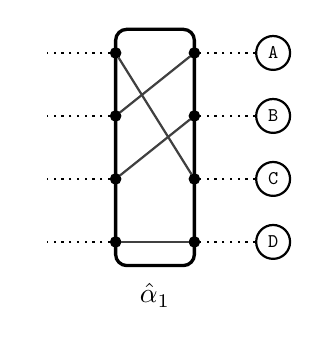
\begin{tikzpicture}
            \tikzstyle{connect}=[circle, draw, thin,fill=black, scale=0.4]
            \tikzstyle{every path}=[thick]
            \tikzstyle{rotor}=[very thick,rounded corners]
            \tikzstyle{input}=[circle,draw,scale=.7]
            \tikzstyle{internalwire}=[thick,darkgray]

            % rotors
            \draw[rotor] (0,0) rectangle (1,3);
            \node[below] at (.5,-.1) {$\hatalpha_1$};

            % first rotor nodes
            \node[connect] (r1r1) at (1,2.7) {};
            \node[connect] (r1r2) at (1,1.9) {};
            \node[connect] (r1r3) at (1,1.1) {};
            \node[connect] (r1r4) at (1,.3) {};
            \node[connect] (r1l1) at (0,2.7) {};
            \node[connect] (r1l2) at (0,1.9) {};
            \node[connect] (r1l3) at (0,1.1) {};
            \node[connect] (r1l4) at (0,.3) {};

            % first rotor wires
            \draw[internalwire] (r1r1) to (r1l2);
            \draw[internalwire] (r1r2) to (r1l3);
            \draw[internalwire] (r1r3) to (r1l1);
            \draw[internalwire] (r1r4) to (r1l4);

            % phantom nodes
            \node (rfr1) at (-1,2.7) {};
            \node (rfr2) at (-1,1.9) {};
            \node (rfr3) at (-1,1.1) {};
            \node (rfr4) at (-1,.3) {};

            % input letters
            \node[input] (Ain) at (2,2.7) {$\mathtt{A}$};
            \node[input] (Bin) at (2,1.9) {$\mathtt{B}$};
            \node[input] (Cin) at (2,1.1) {$\mathtt{C}$};
            \node[input] (Din) at (2,.3) {$\mathtt{D}$};

            % connecting wires
            \draw[dotted] (Ain) -- (r1r1);
            \draw[dotted] (Bin) -- (r1r2);
            \draw[dotted] (Cin) -- (r1r3);
            \draw[dotted] (Din) -- (r1r4);

            \draw[dotted] (r1l1) -- (rfr1);
            \draw[dotted] (r1l2) -- (rfr2);
            \draw[dotted] (r1l3) -- (rfr3);
            \draw[dotted] (r1l4) -- (rfr4);
        \end{tikzpicture}
        & \quad
        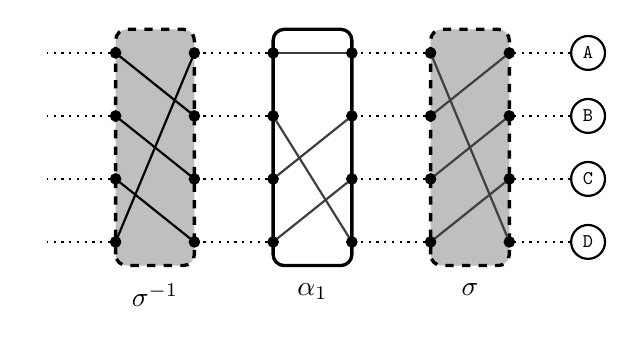
\begin{tikzpicture}
            \tikzstyle{connect}=[circle, draw, thin,fill=black, scale=0.4]
            \tikzstyle{every path}=[thick]
            \tikzstyle{rotor}=[very thick, rounded corners]
            \tikzstyle{shiftperm}=[very thick, dashed, rounded corners, fill=lightgray]
            \tikzstyle{input}=[circle,draw,scale=.7]
            \tikzstyle{internalwire}=[thick,darkgray]

            % rotors
            \draw[shiftperm] (2,0) rectangle (3,3);
            \node[below] at (2.5,-.1) {$\sigma^{-1}$};
            \draw[rotor] (4,0) rectangle (5,3);
            \node[below] at (4.5,-.1) {$\alpha_1$};
            \draw[shiftperm] (6,0) rectangle (7,3);
            \node[below] at (6.5,-.1) {$\sigma$};

            % first rotor nodes
            \node[connect] (r1r1) at (7,2.7) {};
            \node[connect] (r1r2) at (7,1.9) {};
            \node[connect] (r1r3) at (7,1.1) {};
            \node[connect] (r1r4) at (7,.3) {};
            \node[connect] (r1l1) at (6,2.7) {};
            \node[connect] (r1l2) at (6,1.9) {};
            \node[connect] (r1l3) at (6,1.1) {};
            \node[connect] (r1l4) at (6,.3) {};
            % first rotor wires
            \draw[internalwire] (r1r1) to (r1l2);
            \draw[internalwire] (r1r2) to (r1l3);
            \draw[internalwire] (r1r3) to (r1l4);
            \draw[internalwire] (r1r4) to (r1l1);

            % second rotor nodes
            \node[connect] (r2r1) at (5,2.7) {};
            \node[connect] (r2r2) at (5,1.9) {};
            \node[connect] (r2r3) at (5,1.1) {};
            \node[connect] (r2r4) at (5,.3) {};
            \node[connect] (r2l1) at (4,2.7) {};
            \node[connect] (r2l2) at (4,1.9) {};
            \node[connect] (r2l3) at (4,1.1) {};
            \node[connect] (r2l4) at (4,.3) {};
            % second rotor wires
            \draw[internalwire] (r2r1) to (r2l1);
            \draw[internalwire] (r2r2) to (r2l3);
            \draw[internalwire] (r2r3) to (r2l4);
            \draw[internalwire] (r2r4) to (r2l2);

            % third rotor nodes
            \node[connect] (r3r1) at (3,2.7) {};
            \node[connect] (r3r2) at (3,1.9) {};
            \node[connect] (r3r3) at (3,1.1) {};
            \node[connect] (r3r4) at (3,.3) {};
            \node[connect] (r3l1) at (2,2.7) {};
            \node[connect] (r3l2) at (2,1.9) {};
            \node[connect] (r3l3) at (2,1.1) {};
            \node[connect] (r3l4) at (2,.3) {};
            % third rotor wires
            \draw (r3r1) to (r3l4);
            \draw (r3r2) to (r3l1);
            \draw (r3r3) to (r3l2);
            \draw (r3r4) to (r3l3);  

            % phantom reflector nodes
            \node (rfr1) at (1,2.7) {};
            \node (rfr2) at (1,1.9) {};
            \node (rfr3) at (1,1.1) {};
            \node (rfr4) at (1,.3) {};


            % input letters
            \node[input] (Ain) at (8,2.7) {$\mathtt{A}$};
            \node[input] (Bin) at (8,1.9) {$\mathtt{B}$};
            \node[input] (Cin) at (8,1.1) {$\mathtt{C}$};
            \node[input] (Din) at (8,.3) {$\mathtt{D}$};

            % connecting wires
            \draw[dotted] (r1l1) -- (r2r1);
            \draw[dotted] (r1l2) -- (r2r2);
            \draw[dotted] (r1l3) -- (r2r3);
            \draw[dotted] (r1l4) -- (r2r4);

            \draw[dotted] (r2l1) -- (r3r1);
            \draw[dotted] (r2l2) -- (r3r2);
            \draw[dotted] (r2l3) -- (r3r3);
            \draw[dotted] (r2l4) -- (r3r4);

            \draw[dotted] (r3l1) -- (rfr1);
            \draw[dotted] (r3l2) -- (rfr2);
            \draw[dotted] (r3l3) -- (rfr3);
            \draw[dotted] (r3l4) -- (rfr4);


            \draw[dotted] (Ain) -- (r1r1);
            \draw[dotted] (Bin) -- (r1r2);
            \draw[dotted] (Cin) -- (r1r3);
            \draw[dotted] (Din) -- (r1r4);
        \end{tikzpicture}
    \end{tabular}
\end{center}
\caption{Writing the effect of rotation of a rotor as a conjugation by the
``shift forward'' permutation $\sigma$. The permutations diagrammed on the left
and right are equal.}
\label{fig:rotate}
\end{figure}


\subsection{The Types of $\Delta_i$}

The next key observation in understanding the behavior of an Enigma machine is
that, at any given time, the machine will compute a permutation on the letters
that has a specific type, namely $[2^{13}]$. In other words, the permutation
computed will always be the product of $13$ disjoint cycles of length $2$. This
will follow easily from the results of the previous section, plus the
observation that the reflector $\rho$ is wired to never map a letter to itself.

We generalize the type of permutation under consideration to any even size
alphabet.
\begin{definition}
    Let $|\Sigma|$ be even. A permutation on $\Sigma$ is called a
    \emph{reflector} if it has type $[2^{n/2}]$.
\end{definition}
These permutations are more commonly called \emph{proper involutions}.
(A \emph{(non-proper) involution} is a permutation with cycle decomposition
consisting of cycles of length of $1$ or $2$, i.e. type $[1^{z_1}2^{z_2}]$
for some $z_1,z_2$.)

\begin{lemma}
    Let $|\Sigma|$ be even and $\rho$ be a reflector on $\Sigma$.
    Then the following hold:
    \begin{itemize}
        \item $\rho^{-1}=\rho$,
        \item For all $x\in\Sigma$, $\rho(x)\neq x$.
    \end{itemize}
\end{lemma}
    \begin{exercise} Prove this lemma. The reverse direction also holds; Prove that as well.
    \end{exercise}

\begin{lemma}\label{lem:deltarefl}
    Let $\Delta_i$ be the permutation computed by the simplified Engima machine
    at step $i$, as defined in Equation~(\ref{eq:enigmaperm1}). Then $\Delta_i$
    is a reflector.
\end{lemma}
\begin{proof}
    We showed above that $\Delta_i$ is a conjugate of $\rho$, and by
    Corollary~\ref{cor:conjtype}, $\Delta_i$ has the same type as the reflector
    $\rho$, i.e. type $[2^{n/2}]$.  Thus $\Delta_i$ is a reflector.
\end{proof}

\section{Rejewski's Theorem and Attack}

Rejewski's attack assumes it is given several ciphertexts generated with
message keys chosen by senders; It will recover those message keys with only a
little effort. In fact, the attack is efficient enough to do by hand!

The attack proceeds in three steps:
\begin{enumerate}

    \item Use the ciphertexts to compute the entire tables (or cycle
        decomposition) of the permutations $\Delta_4\Delta_1,\Delta_5\Delta_2$,
        and $\Delta_6\Delta_3$.
    \item Find all possible factorizations of $\Delta_4\Delta_1$,
        $\Delta_5\Delta_2$, and $\Delta_6\Delta_3$ into products of two
        reflectors.
    \item From amongst the possible factorizations, figure out which
        ones are the correct ones, and hence learn $\Delta_1,\Delta_2,\Delta_3$.
        Now message keys can be recovered .
\end{enumerate}

\subsection{Step One: Learning $\Delta_4\Delta_1,\Delta_5\Delta_2$,
        and $\Delta_6\Delta_3$}

This step is based on the following lemma:
\begin{lemma}\label{lem:repeats}
    Let $\rho_1$ and $\rho_2$ be reflectors on $\Sigma$.
    Then for $x\in\Sigma$, if $\rho_1(x)=y_1$, and $\rho_2(x)=y_2$, then
    $\rho_2\rho_1(y_1)=y_2$.
\end{lemma}
\begin{proof}
    Since $\rho_1$ is a reflector and $\rho_1(x)=y_1$, we have that
    $\rho_1(y_1)=x$. This can been seen in either of two
    ways: First, since $\rho_1$ is a reflector, $\rho_1^{-1}=\rho_1$,
    and
    \[
        \rho_1(x)=y_1 \quad \iff \quad 
        \rho_1^{-1}(\rho_1(x))=\rho_1^{-1}(y_1) \quad \iff \quad 
        x=\rho_1^{-1}(y_1) \quad \iff \quad 
        x=\rho_1(y_1). 
    \]
    Alternatively, we could just observe that since $\rho_1$ is a reflector
    then it must have $(x\ y_1)$ in its cycle decomposition.

    Finally, using $\rho_1(y_1)=x$ we get
    \[
        \rho_2\rho_1(y_1) = 
        \rho_2(x) = y_2,
    \]
    as desired.
\end{proof}

Here is an example of how it is used against a single ciphertext:
\begin{example}
Suppose we observe a ciphertext starting with $\mathtt{ICPWLV}$. We know
that there exist $x,y,z\in\Sigma$ such that
\[
\mathtt{ICPWLV} = \Delta_1(x)\Delta_2(y)\Delta_3(z)
    \Delta_4(x)\Delta_5(y)\Delta_3(z),
\]
where the $\Delta_i$ are unknown permutations computed by the Enigma machine.
We do however know that they are all reflectors, by
Lemma~\ref{lem:deltarefl}.  Applying Lemma~\ref{lem:repeats}, we can infer
that
\[
    \Delta_4\Delta_1(\mathtt{I})=\mathtt{W},
    \quad \quad
    \Delta_5\Delta_2(\mathtt{C})=\mathtt{L},
    \quad and \quad
    \Delta_6\Delta_3(\mathtt{P})=\mathtt{V}.
\]
\end{example}

To learn all of $\Delta_4\Delta_1,\Delta_5\Delta_2$, and $\Delta_6\Delta_3$,
the Polish team would look over many ciphertexts. Each ciphertext would
tell them how one letter is mapped in each of the products; After enough time,
they would typically see how all of the letters are mapped by each product.
This completes step one.

\subsection{Step Two: Factoring $\Delta_4\Delta_1,\Delta_5\Delta_2$,
        and $\Delta_6\Delta_3$}

Now we assume we know the products, and want to recover the individual
$\Delta_i$. Rejewski based this step on the following theorem:
\begin{theorem}[Rejewski]\label{thm:rejewski}
    Let $\rho_1$ and $\rho_2$ be reflectors on $\Sigma$.  Then if $(a_1\ a_2\
    \cdots\ a_t)$ appears in the cycle decomposition of their product
    $\rho_2\rho_1$, the cycle
    \[
        (\rho_1(a_t)\ \rho_1(a_{t-1})\ \cdots\ \rho_1(a_1))
    \]
    also appears in the cycle decomposition of $\rho_2\rho_1$, and moreover
    this cycle is distinct from $(a_1\ a_2\ \cdots\ a_t)$.
\end{theorem}
We will prove this theorem in the last section. For now we state an
interesting corollary and then show how to apply the theorem.
\begin{corollary}
    Let $\rho_1$ and $\rho_2$ be reflectors, and let $[1^{z_1}2^{z_2}\cdots
    n^{z_n}]$ be the type of their product $\rho_2\rho_1$. Then all of the
    $z_i$ are even.
\end{corollary}
\begin{exercise}
    Prove the corollary.
\end{exercise}

This lemma is applied once one has the cycle decomposition of
$\Delta_4\Delta_1$ from the previous step. By the lemma, we know that the
cycles must appear in pairs, where one cycle in the pair is the reverse of the
other with $\Delta_1$ applied to each element. If we knew exactly how the
cycles were paired up, we could just read off the values of $\Delta_1$.
Unfortunately we \emph{don't} know how exactly how they pair up, but it
will turn out that there aren't usually too many ways they could pair up.
In the next step we'll figure out which is the correct one.

\begin{example}
    Suppose we have determined that
    \[
        \Delta_4\Delta_1 = (\mathtt{OGKRYSD})(\mathtt{ZUQWFIB})
        (\mathtt{MJXCP})(\mathtt{HLNVE})(\mathtt{A})(\mathtt{T}).
    \]
    This is the type of cycle decomposition predicted by the Theorem:
    We have a pair of cycles of length $7$, a pair of size $5$,
    and a pair of size $1$. Since there are only two cycles of each
    length, we know how they must pair up. But we don't know how to
    cyclically align them as the theorem says. For instance, we may
    pair up
    \[
        (\mathtt{OGKRYSD})(\mathtt{ZUQWFIB}) = 
        (\mathtt{OGKRYSD})(\Delta_1(\mathtt{D})\cdots\Delta_1(\mathtt{G})\Delta_1(\mathtt{O}))
    \]
    and guess that $\Delta_1(\mathtt{O}) = \mathtt{B}, \Delta_1(\mathtt{G}) =
    \mathtt{I}$, etc. (Note that we wrote the cycles of size one here to
    emphasize their presence.) Alternatively, the cycles may also be written
    \[
        (\mathtt{OGKRYSD})(\mathtt{UQWFIBZ})
        =
        (\mathtt{OGKRYSD})(\Delta_1(\mathtt{D})\cdots\Delta_1(\mathtt{G})\Delta_1(\mathtt{O}))
    \]
    in which case we would guess that $\Delta_1(\mathtt{O}) = \mathtt{Z},
    \Delta_1(\mathtt{G}) =\mathtt{B}$, etc.
    Each of the $7$ possible rotations generates a different guess for
    that part of $\Delta_1$. The same issue happens with the
    cycles of size $5$. With the $1$-cycles there is thankfully no
    ambiguity.
\end{example}
\begin{example}\label{ex:sixcycles} A further complication comes up when $\Delta_4\Delta_1$
    has more than two cycles of a given length. For instance, if
    \[
        \Delta_4\Delta_1 = (\mathtt{AILNMC})(\mathtt{RGYBOF})
        (\mathtt{WZESQU})(\mathtt{DHVXJP})(\mathtt{K})(\mathtt{T}),
    \]
    then we have to decide how to pair up the cycles of size $6$,
    and there are $3$ different ways doing so; After pairing them
    up, we again of $6$ ways of rotating each pair independently.
\end{example}

\begin{exercise}
    Suppose $\Delta_4\Delta_1$ has type $[1^{z_1}2^{z_2}\cdots n^{z_n}]$. Give
    a formula (in terms of the $z_i$) for the number of factorizations that the
    process above will give. Can you find the type that maximizes that number?
\end{exercise}

\subsection{Step Three: Identifying $\Delta_1,\Delta_2$, and $\Delta_3$}

The previous step generates several guesses for the $\Delta_i$. To
determine which is most likely the correct one, the team would exploit
the fact that senders sometimes chose non-random message keys. Message
keys like $\mathtt{AAA},\mathtt{BBB},\mathtt{ABC}$, etc were chosen
by operators, and these characteristics enabled a limited form of 
frequency analysis. An easy property is that the first character of the
message key was most frequently $\mathtt{A}$; This yields a guess for
$\Delta_1(\mathtt{A})$, and then the above technique will extend it to
guess the rest of cycle containing $\mathtt{A}$.
\begin{exercise}
    Let $\Delta_4\Delta_1$ be as in Example~\ref{ex:sixcycles}, and suppose
    you observe that the most frequent first letter of message keys is
    $\mathtt{Y}$. What values of $\Delta_1$ does this lead you to guess?
\end{exercise}
This process takes some guesswork, but is reported to have worked well.
It helped that a guess could be checked, because even less frequent message
keys would often have some structure (like $\mathtt{HIJ}$), and these would
appear once the correct permutations had been recovered.

\subsection{Proof of Rejewski's Theorem (Optional)}

Let $\rho_1$ and $\rho_2$ be reflectors, and suppose $(a_1\ a_2\ \cdots\ a_t)$
appears in the cycle decomposition of their product $\rho_2\rho_1$. We need to
show that   $(\rho_1(a_t)\ \rho_1(a_{t-1})\ \cdots\ \rho_1(a_1))$ also
appears and is distinct.

Start by writing $\rho_1(a_i) = b_i$ for $i=1,\ldots,t$.
Since $\rho_1$ is a reflector we also have that $\rho_1(b_i) = a_i$.
We claim that none of
the $b_i$ will equal any $a_j$ (more formally, that $\{a_1,\ldots,a_t\}$ and
$\{b_1,\ldots,b_t\}$ are disjoint sets). We'll assume that's true for now and
finish proving the theorem, and then come back to verify that fact at the end.

Since $\rho_2\rho_1(a_i) = a_{i+1\bmod t}$, we must have $\rho_2(b_i) =
a_{i+1\bmod t}$; Again since $\rho_2$ is a reflector, we have
$\rho_2(a_i) = b_{i-1\bmod t}$ for all $i=1,\ldots,t$ (note that we swapped up
the subscript to subtract on one side instead of add to the other side, but
this still true for general $i$).  Then
\[
    \rho_2\rho_1(b_i) = 
    \rho_2(a_i) = b_{i-1\bmod t}.
\]
In other words, we have shown that $\rho_2\rho_1$ maps $b_i$ to $b_{i-1\bmod
t}$, i.e. $\rho_1(a_i)$ to $\rho_1(a_{i-1\bmod t})$. This is exactly what we
wanted to show.\qed

We now return to the claim that $\{a_1,\ldots,a_t\}$ and 
$\{\rho_1(a_1),\ldots,\rho_1(a_t)\}$
are disjoint sets. 
This will follow from the following lemma. 
\begin{lemma}
    Suppose $\rho_1$ and $\rho_2$ are reflectors and that $\rho_1(x)=y$.
    Then $x$ and $y$ are in different cycles in the decomposition of
    $\rho_2\rho_1$.
\end{lemma}
\begin{proof}
    To show that $x$ and $y$ are in different cycles of $\rho_2\rho_1$, it
    suffices to show that $(\rho_2\rho_1)^k(x) \neq y$ for every $k\geq 1$.
    For any $k\geq 1$ we have
    \[
        (\rho_2\rho_1)^k(x)
        = (\rho_2\rho_1)^{k-1}\rho_2\rho_1(x)
        = (\rho_2\rho_1)^{k-1}\rho_2(y).
    \]
    We need to show that $(\rho_2\rho_1)^{k-1}\rho_2(y)\neq y$. We'll do this
    by showing that $(\rho_2\rho_1)^{k-1}\rho_2$ is a reflector.
    This follows by checking that $(\rho_2\rho_1)^{k-1}\rho_2$ is actually
    a conjugate of either $\rho_1$ or $\rho_2$ for every $k\geq 1$. For
    example, if $k=1$ this is just $\rho_2$. If $k=2$ then
    \[
        (\rho_2\rho_1)^{2-1}\rho_2 = \rho_2\rho_1\rho_2 = 
         \rho_2\rho_1\rho_2^{-1}, 
    \]
    which is a conjugate of $\rho_1$ and hence a reflector. Working out
    the exact formula is left as an exercise.
\end{proof}



\end{document}

